\documentclass{article}
\usepackage{../../pset}

\title{Adaptive Metropolis Hastings}
\author{Brian Shimanuki}

\begin{document}
\maketitle

\begin{abstract}

I will be implementing an online-adaptive MCMC algorithm in order to infer a matching set of rectangles to an observed image. The main focus will be to replicate \cite{dippl} and extend Metropolis-Hastings to use adaptive inference parameters. To ensure that the convergence properties still hold, the adaptation will diminish over time.

I will use a prior on the latent structure which encodes rectangles of random sizes, orientations, colors, and opacities. The negative log likelihood of a sample will be the $\ell_1$ norm of the difference between the observed image and the image corresponding to the latent parameters. The transition distribution will be a Guassian with an adaptive standard deviation.

The main results will be to compare Metropolis-Hastings both with and without adaptive parameters on a set of images.

\end{abstract}

\begin{figure}[h]
	\centering
	\begin{tabular}{lccc}
		& $l=1$ & $l=10$ & $l=100$ \\
		$\sigma=0.1$
		& 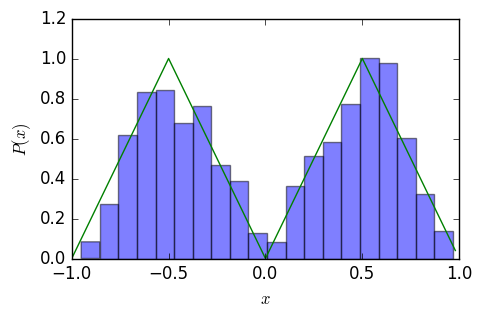
\includegraphics[valign=m,width=1.3in]{{plots/doublepeak1_0.1}.png}
		& 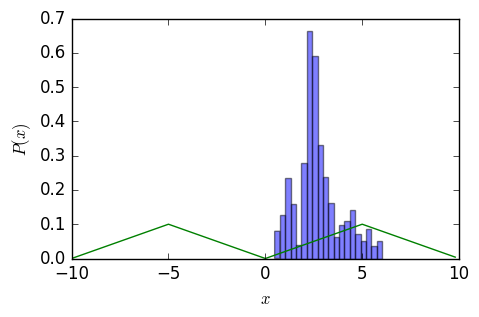
\includegraphics[valign=m,width=1.3in]{{plots/doublepeak10_0.1}.png}
		& 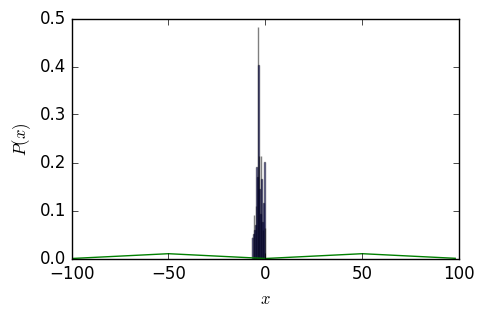
\includegraphics[valign=m,width=1.3in]{{plots/doublepeak100_0.1}.png}
		\\
		$\sigma=1$
		& 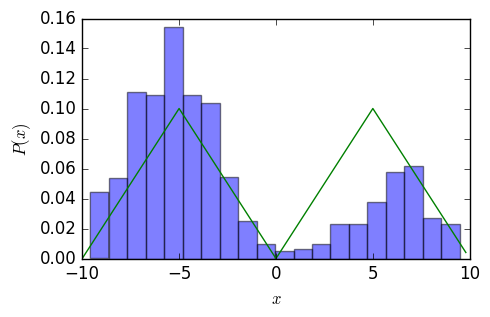
\includegraphics[valign=m,width=1.3in]{{plots/doublepeak10_1}.png}
		& 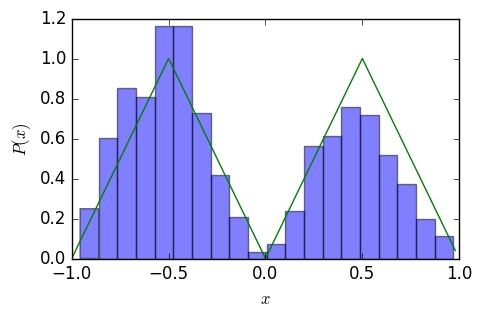
\includegraphics[valign=m,width=1.3in]{{plots/doublepeak1_1}.png}
		& 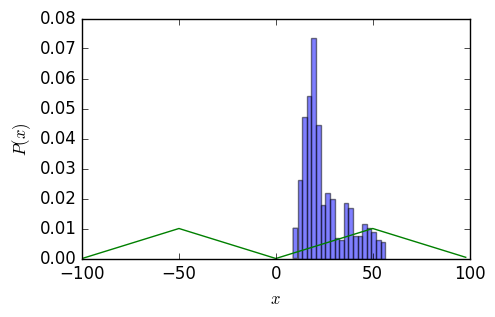
\includegraphics[valign=m,width=1.3in]{{plots/doublepeak100_1}.png}
		\\
		$\sigma=10$
		& 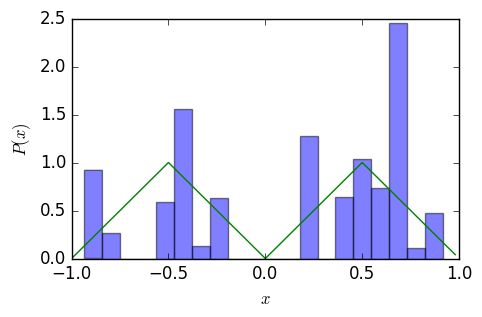
\includegraphics[valign=m,width=1.3in]{{plots/doublepeak1_10}.png}
		& 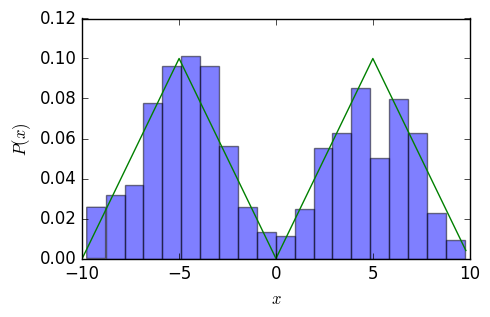
\includegraphics[valign=m,width=1.3in]{{plots/doublepeak10_10}.png}
		& 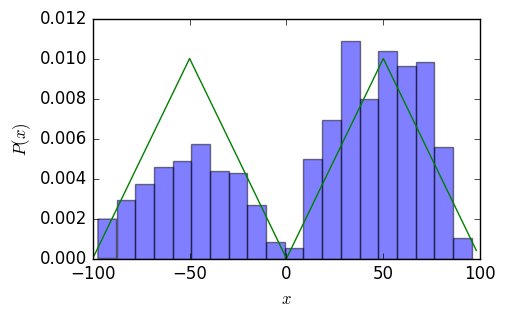
\includegraphics[valign=m,width=1.3in]{{plots/doublepeak100_10}.png}
		\\
		Adaptive
		& 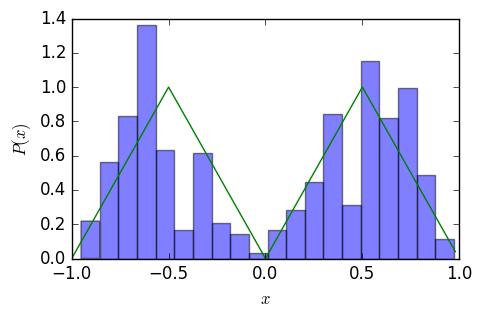
\includegraphics[valign=m,width=1.3in]{{plots/doublepeak1_adaptive}.png}
		& 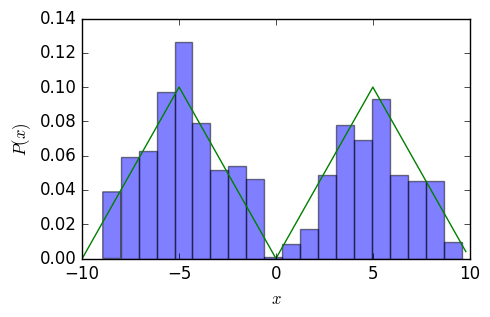
\includegraphics[valign=m,width=1.3in]{{plots/doublepeak10_adaptive}.png}
		& 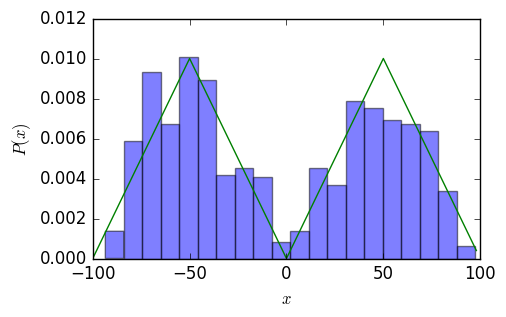
\includegraphics[valign=m,width=1.3in]{{plots/doublepeak100_adaptive}.png}
	\end{tabular}
	\caption{5000 samples (Burn-in 1000) of $p(x)=\max(\min(|x|,l-|x|),0)$}
	\label{fig:peaks}
\end{figure}

\nocite{*}
\bibliographystyle{acm}
\bibliography{bibliography}

\end{document}
